\footnotetext[1]{A dragon which gnaws at the roots of Yggdrasil, the world tree, in Norse mythology.}
\footnotetext[2]{Messenger squirrel who runs up and down Yggdrasil.}
\footnotetext[3]{The afterlife for murderers, adulterers and oath-breakers (the worst possible crimes in Viking society).}

The realms were vast beneath my wings as the winds carried me. They took me from the gleaming city of Asgard, with its impressive walls and gods combined, to the very roots of Yggdrasil where Niddhog\footnotemark[1] lay in wait. I raced old Ratatosk\footnotemark[2] from where he perched and felt the suns and worlds breathe beneath like pulsing waves. In the darkest corner of the universe, lay a bridge between the forests of the living and the dead. At its gates sat dearest Garm, a splendid hound, who guarded the realm of the living from the dead. 

She glanced up at me, grunted in recognition, and lay down in front of the gate. She lolled her head to the side and watched the colourless dead enter her realm. They walked in groups sometimes, and some came on their own. Some were haggard from a painful life; some appeared splendid in their colourful gowns. Some even toddled through the crowds with no one to hold onto, their helpless faces scrunched with fear and worry. And those, kind Garm would pick up on her paws, and carry to their new homes. Some of those who ventured in beamed gratefully at her. Others still, glared daggers at the world they would have to call home. They flexed their fingers itching for weapons left behind with their living bodies.
 
I perched upon the gates and watched their lulling walks with mild disinterest, taking in the vast expanse of the realm. Within Helheim, among the masses of people walking peacefully, a man and woman cowered in fear as they were ushered towards Nastrond\footnotemark[3] by those dead that Hel entrusted with responsibilities. The couple's eyes darted around nervously. 

I tilted my head and waited.

They held onto each other but the man ducked behind the woman, using her as a shield. I glanced over at Garm, but she appeared nonplussed. She inclined her head to watch a cave in Nastrond, and hummed. 

The woman screamed.

A mighty dragon appeared from the confines of the cave, its wings spreading as wide as five longboats, as it flew over Nastrond. It flew up as far as it could before the chains around its tail began to strain, and it delved down like a cormorant. It plucked the couple into its mouth, and the screams came to a crunching end. With that, Niddhog swiftly escaped back into his midnight cave, and only his eyes gleamed in the darkness, oozing with a vengeful, hungry heart. He stared at me, and I could see an angry cloud of fire leave its nostrils in frustration.

\footnotetext[1]{The river that separates the living from the dead.}
\footnotetext[2]{The horse ridden by Odin, and child of Loki- a trickster figure in Norse myths.}

I am not his meal just yet.

I cawed a farewell to Garm, and flew over the dark realm, weaving through the winds which blew into Helheim from the river Gj{\"o}ll\footnotemark[1]. The dead were as they lived, farming, serving, existing as they had before. Helheim was no eternal place of rest, and it was no eternal place of revelry. Indeed, it was just like all the other realms, with only the barest distinction that all permanent inhabitants but one were wholly dead. I flew past farms and towns and markets. I flew quickly but memorised the land once more, seeking out any significant changes. I found naught. 

I dove low as I encroached the palace grounds, and saw horses graze on a splendid meadow outside magnificent wooden stables. There were a dozen mares watching three spindly foals prance and play. The stallions watched on from within the stables, their attendants unwilling to risk having to care for more foals just yet. Among these stallions, however, was one like none other. A speckled grey stud with a fiery red mane drank water brought to it by an attendant. He kicked two of his hind legs, as he balanced on his other six, whinnying with satisfaction after a long ride well done. 

I cawed at Sleipnir\footnotemark[2] as I flew by, but he did not hear me. I travelled on.

Before long, I flit into the palace with my little raven wings and knew that I was in the very heart of the realm. I flew along the ceiling made of indigenous, dark materials which sucked out all light incident upon them, content in the knowledge that I was concealed from prying eyes. I swooped through the halls with ease for there were few doors in the palace. After all, doors are but for safety and there is no need for barriers within a place that needs no protection. The dead cannot die again, and no harm can befall the realm, especially under the rule of the auspicious Queen. 

I circled the eastern wing a couple times, where countless men, women, and children of all races and realms awaited care in an infirmary. The Queen's attendants walked in with new patients at all hours of all days, for there was never a shortage of the infirm to wander through death's door.  While many required continual care and attention, some merely needed their axe wounds stitched up once more. The attendants, once healers in their other lives, worked diligently through every night and every day, slowly restoring health and even a little youth to their patients with almost a devout love. They served and cared for their patients with tenderness, even those into whose skulls they might wish to bury one more crushing axe. For pleasing the Queen was, after all, tantamount to saving a life in another realm. And nothing pleased the Queen more than when the healed left the palace and took up professions in her lands. Or so they gladly believe.

At last, I left, dashing in and out of several rooms searching for the woman that ruled them all. I dove into the Queen's chambers, sought out the great hall where seemingly endless audiences took place, weaved carefully through the potions rooms and even bobbed briefly into the servants' quarters. But she was nowhere to be found. I cawed to myself in annoyance and turned a corner into another empty hall, continuing my hunt. After exhausting nearly all possibilities, I found the hall where her blackened locks glimmered, framing her half skeletal face.

\footnotetext[1]{Son of Odin and Frigg. He was killed by a spear of mistletoe in a plot by Loki.}

She sat at the centre of the head table, in a feasting hall brimming with her peoples. Each of the tables was stacked high with succulent meats of livestock reared by dead farmers, and darkly shaded vegetation grown within the realm. Some of the dead were hunched over their platters devouring food so fast they would have died in their recklessness elsewhere. Others took more care and savoured the feasts, relishing flavours like they were a gift they had not received in multiple lifetimes. Yet others, who could barely move their wooden utensils to their lips, were fed by their patient attendants. Though there were no endless fountains of mead or drunken warriors who had died gloriously in battle, there was no shortage of merriment in the Queen's hall. Ale spilled everywhere as greatly exaggerated tales of valour in glory days long past were shared amongst the many healing.

Though raucous laughter echoed through parts of the hall, many were not partaking in the revelry, as they looked upon the guest of honour. Even young ones who knew nothing of the legends of the living looked upon him with a curious love blossoming in their hearts, for Balder the beloved\footnotemark[1] was amongst them. Men and women alike swooned at the beautiful man, coveting him in their hearts. If the Queen were not there they would have gathered at his feet, eager to touch him and claim even a single hair on his head as their own.  He nodded politely at all who managed to catch his attention but simply continued speaking with his brother, Hermod, whose skin was not stained with death.

I watched the proceedings in silence, distaste in my mouth at the reverence given to the foolish man. I was ever so tempted to leave a pungent dropping on his hair. 

Before any plans of action could be put into practice, the hall fell into silence as the Queen rose. None dared to move a muscle, but for young Hermod, who looked around in confusion. She smiled blankly at the guests of honour, and turned on her heel. She left as only a true queen could, her moss green dress billowing, sweeping the floor behind her. Once gone, the chatter resumed as if nothing had occurred. 

I flew after her, following the sound of clanging heels in the lightless halls. I glided into her chambers and sat on the edge of her bed, nestling contently on the warm furs. She stood by her commode, with her back to me, and poured mead into two goblets with the slow flow of a woman who knew exactly what she wanted. 

`Come here if you wish to drink with me,' she said simply, not deigning to turn around, as she filled the second goblet. She held one out to me and waited. I jumped off the bed and came to perch upon her outstretched arm. 

I glanced up at her and tilted my head.

`I have no reason to poison you,' Hel murmured with a small chuckle, and took a sip of her own goblet, not taking her eyes off of me. I cawed in thanks and plunged my beak into the sweet mead, drinking with surprised eagerness. It had been a long flight from Asgard, and not even I had realised how much I craved to wet my throat.

She smiled to herself, and walked over to the vanity, with me still slurping away on her arm. She sat down and set the goblet down as well once I was done with the intoxicating nectar of the gods. I hopped along her arm and sat on her shoulder, pushing her hair aside. Our eyes locked in the reflection. 

`I appreciate the gift that has been bestowed upon me this day,' she murmured, not taking her eyes off of me. Her intelligent eyes crinkled with joy, and her lips softened into a smile.

I cawed innocently, and tilted my head, widening my eyes comically.

`It is not every day that Balder the beloved is gifted to me,' she hummed almost dreamily. 

I cawed again, rolling my eyes this time, and poked her cheekbone with my beak.

`Fear not, no single man can enchant me... It is merely pleasant to have what the Allfather\footnotemark[1] covets. That is why they sent unfortunate Hermod to me, is it not? To try and retrieve their beloved little pup?'

\footnotetext[1]{Odin.}
\footnotetext[2]{In Norse mythology, Loki is the father of Hel.}

I nodded in assent. The Allfather was so very predictable sometimes. It was laughable.

`Tell me, shall I return him to the ungrateful lot?' she asked wryly, her lips twisted in amusement.

I made a sound that could only be construed as laughter and shook my head. 

`Perhaps, I shall join in the merriments and play a little game of my own,' she smirked, turning her head to look at me directly. I puffed myself up to be at her eye-level.

`If the Allfather wants him so greatly, I shall return him-?'

I cawed in protest.

`Calm your feathers,' she chuckled and touched the tip of my beak with her forefinger. `I shall return him only if everything in the cosmos weeps for him.' Her face broke into a wide and wicked grin. `I have a feeling I can trust a certain someone to not weep for him, is that not so?'

I stared at her for a few moments and felt pride well up within me. I opened one wing and gently stroked her flesh cheek with it.

Her expression softened and she pressed a kiss to my beak. 

`Good luck with whatever game it is you are playing,' she whispered, her green and blue eyes warm despite the decaying death that surrounded half of her being.

I pecked her flesh cheek tenderly and flew off with a soft caw.

`Be careful, father,' I heard Hel whisper in goodbye\footnotemark[2].

\begin{figure}[h!]
\centering
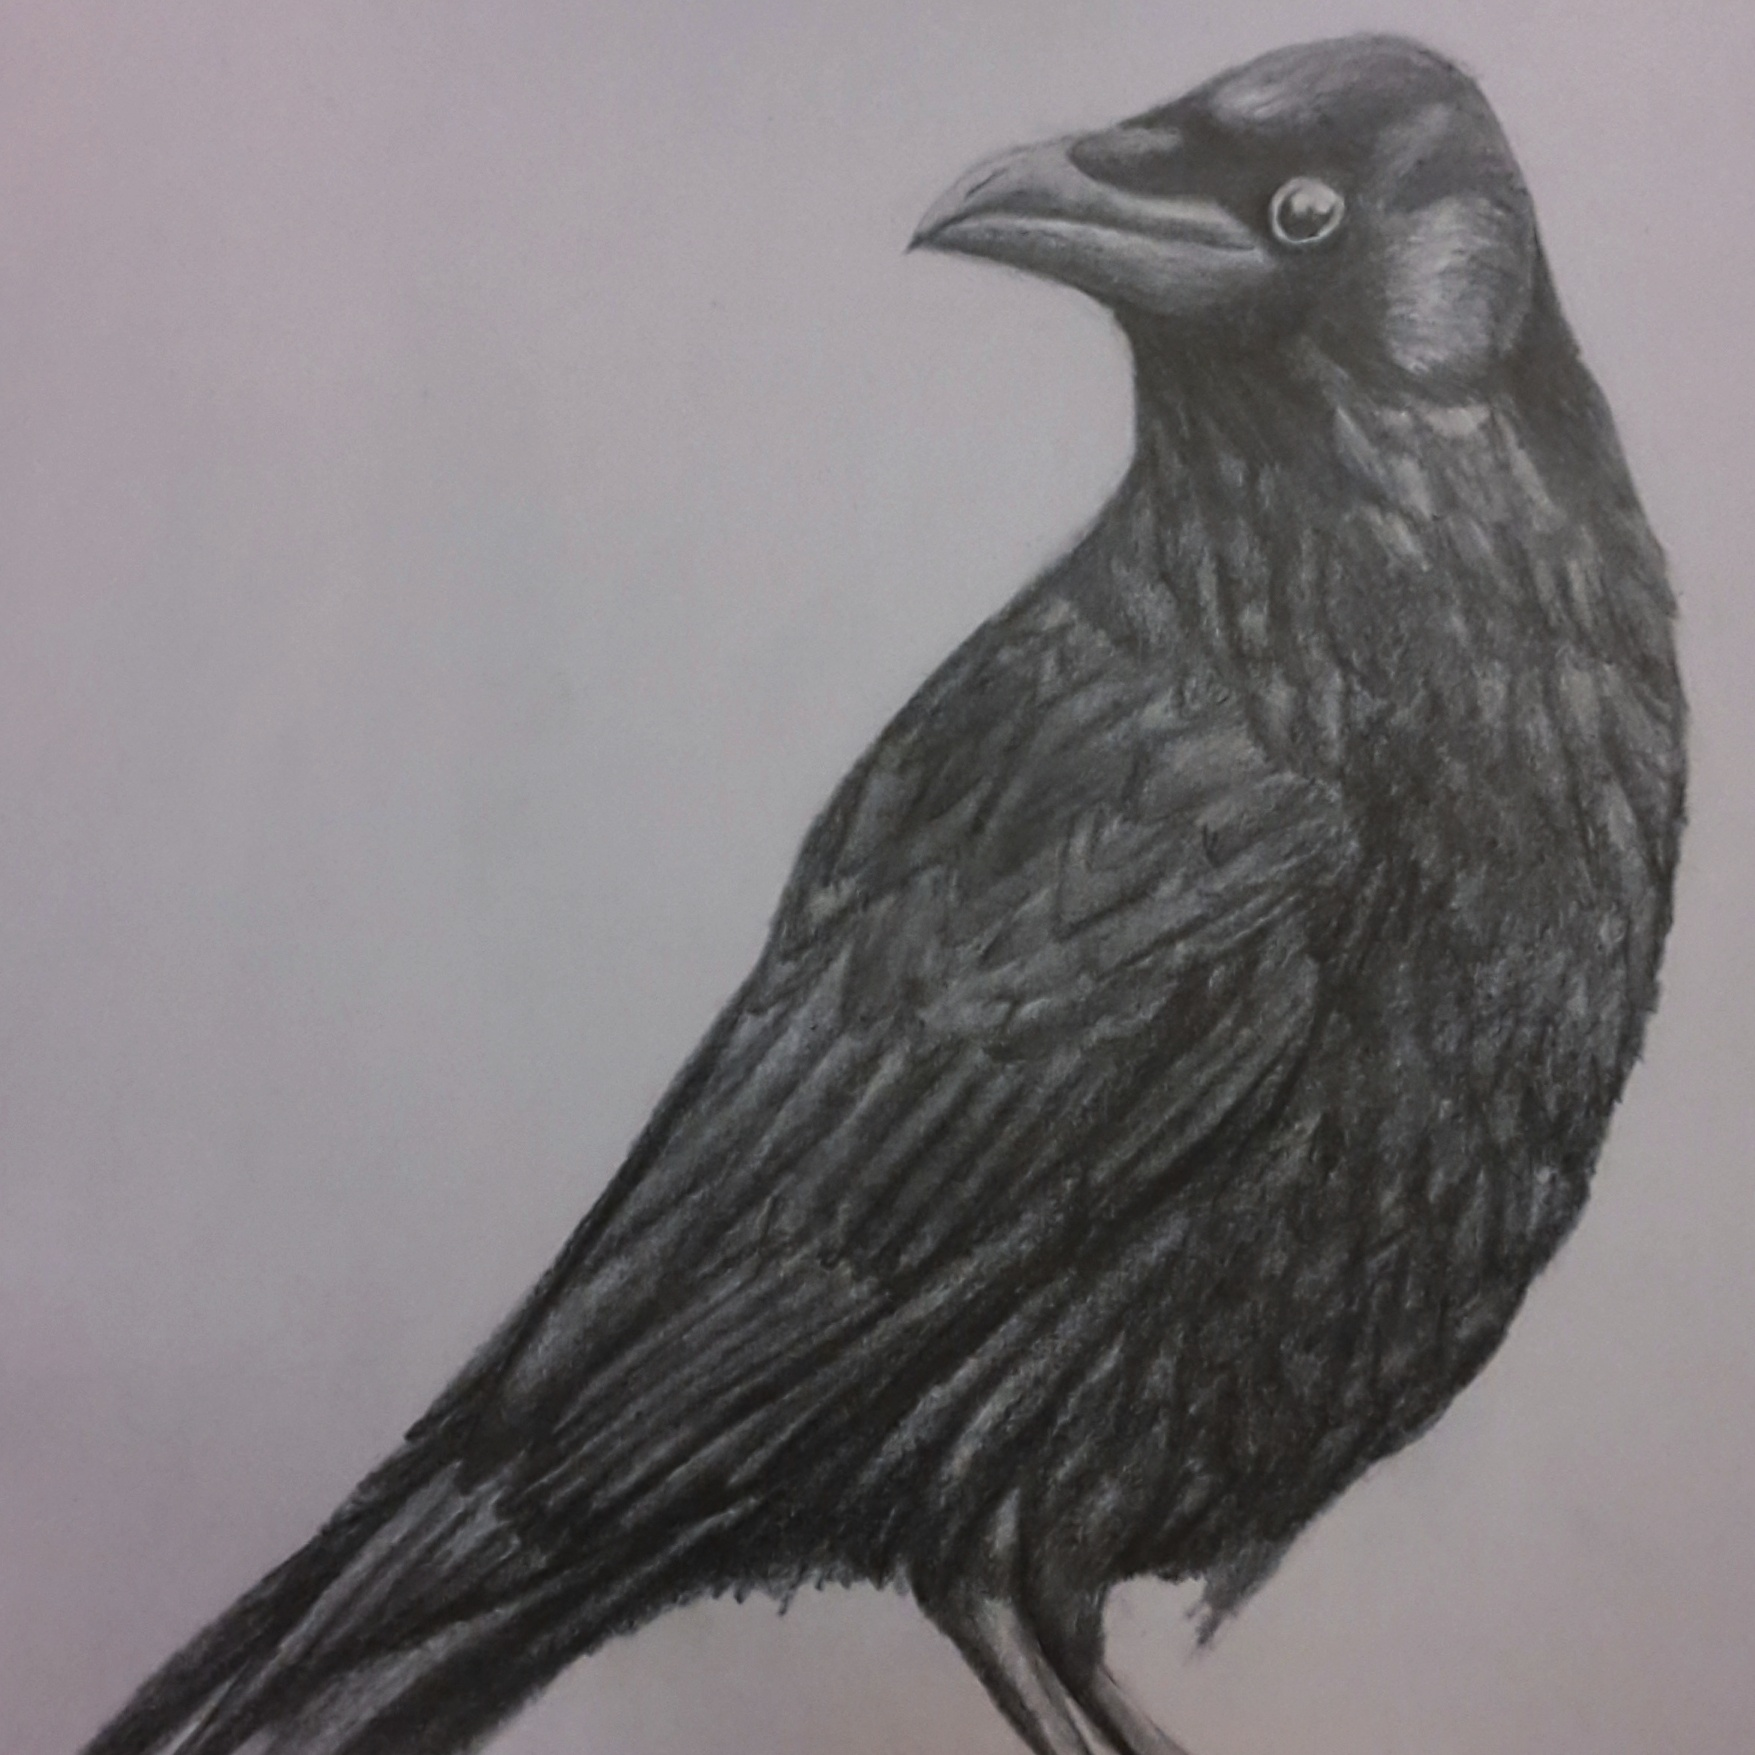
\includegraphics[width=0.9\textwidth]{./pictures/raven}
\end{figure}